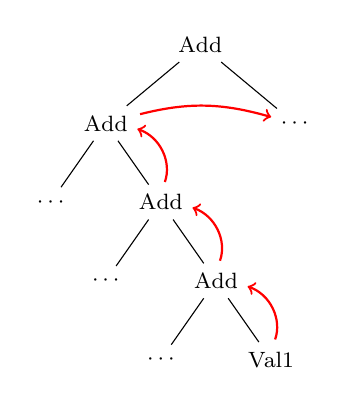
\begin{tikzpicture}
\tikzset{
    ncbar angle/.initial=90,
    ncbar/.style={
        to path=(\tikztostart)
        -- ($(\tikztostart)!#1!\pgfkeysvalueof{/tikz/ncbar angle}:(\tikztotarget)$)
        -- ($(\tikztotarget)!($(\tikztostart)!#1!\pgfkeysvalueof{/tikz/ncbar angle}:(\tikztotarget)$)!\pgfkeysvalueof{/tikz/ncbar angle}:(\tikztostart)$)
        -- (\tikztotarget)
    },
    ncbar/.default=0.5cm,
}

\tikzset{square left brace/.style={ncbar=0.15cm}}
\tikzset{square right brace/.style={ncbar=-0.15cm}}
  \tikzstyle{every node}=[font=\footnotesize]
  \tikzstyle{level 1}=[level distance=10mm, sibling distance=24mm]
  \tikzstyle{level 2}=[level distance=10mm, sibling distance=14mm]
  \tikzstyle{level 3}=[level distance=10mm, sibling distance=14mm]
  \tikzstyle{level 3}=[level distance=10mm, sibling distance=14mm]
  \tikzstyle{load}=[->,thick,color=blue]
  \tikzstyle{unload}=[->,shorten <=1pt,thick,color=red]
	% \draw[step=1cm, very thin, gray] (-6,-6) grid (6,6);
  \node (root) {\AI{Add}}
  child {node (node1) {\AI{Add}} child {node  (node2) {\ensuremath{\cdots}}} 
                                 child {node  (node3) {\AI{Add}} 
                                   child {node  (node4) {\ensuremath{\cdots}}}
                                   child {node  (node5) {\AI{Add}} 
                                                child {node (node8) {\ensuremath{\cdots}}} 
                                                child {node (node7)
                                                {\AI{Val}\AS{}\AN{1}}}}}}
  child {node (node6) {\ensuremath{\cdots}}};

  % \draw[load] (root) to [ bend right=45] (node1);
  % \draw[load] (node1) to [ bend right=45] (node2);
  % \draw[unload] (node2) to [ bend left=15] (node3);
  % \draw[load] (node3) to [ bend right=45] (node4);
  % \draw[unload] (node4) to [ bend left=15] (node5);
  % \draw[load] (node5) to [ loop below] (node5);
  \draw[unload] (node5) to [ bend right=45] (node3);
  \draw[unload] (node3) to [ bend right=45] (node1);
  \draw[unload] (node1) to [ bend left=15] (node6);
  \draw[unload] (node7) to [ bend right=45] (node5);
  % \draw[load] (node6) to [ bend right=45] (node7);
  % \draw[unload] (node7) to [ bend left=15] (node8);
  % \draw[load] (node8) to [ loop below] (node8);
  % \draw[unload] (node8) to [ bend right=45] (node6);
  % \draw[unload] (node6) to [ bend right=45] (root);
  % \draw[step=0.1cm,gray] ($(node2)-(0.2,0.2)$) grid ($(node1)-(0.05,-0.15)$);
  % \draw[step=0.1cm,gray] (node2) grid (node4);
  % \draw[step=0.1cm,gray] (node4) grid (node3);
  % \draw[step=0.1cm,gray] (node2) grid ($(node1)!0.25!(node3)$);
  % \draw[step=0.1cm,gray] (node2) grid ($(node1)!0.5!(node3)$);
  % \draw[step=0.1cm,gray] (node2) grid ($(node1)!0.75!(node3)$);
  % \draw[step=0.1cm,gray] (node4) grid ($(node5)!0.75!(node3)$);
  % \draw[step=0.1cm,gray] ($(node4)-(0.2,0.5)$) grid ($(node5)!0.51!(node3)$);

  % \draw [thick] (-1.5,-5) to [square left brace ] (-1.5,-4);
  % \draw [thick] (3.5,-5) to [square right brace ] (3.5,-4);
	% \node at (-0.75,-4.5) (right1) {{\AI{\color{red}Right}}\AS{}\AN{7},};
	% \node at (0.6,-4.5)    (right2) {{\AI{\color{red}Right}}\AS{}\AN{3},};
  % \node at  (1.75,-4.5) {\AI{\color{blue}Left}};
	% \node at (-2.5, -4.5) {\AN{1}\quad,};
  % \tikzstyle{every node}=[font=\tiny]
  % \tikzstyle{level 1}=[level distance=5mm, sibling distance=7mm]
  % \node at (2.75,-4.25) (left1) {\AI{Add}} 
  %         child {node {\AI{Val}\AS{}\AN{2}}}
  %         child {node {\AI{Val}\AS{}\AN{0}}};

    % \draw [red, thick] (1,0) to [square right brace] (1,4);
\end{tikzpicture}

